\section{Relación entre los espectros basados en la TDF y en espacios monofrecuenciales}

Después de todo lo expuesto en las secciones anteriores, tenemos
ya dos alternativas para realizar un análisis
espectral de una señal $x \in \IR^{n}$.

Sean $n \geq 2$, $M := \lceil \frac{n}{2} \rceil$, $x \in \IR^{n}$.
\begin{itemize}
	\item \textbf{(Espectro-0: basado en la TDF)} 
	Usando la transformada discreta de Fourier
	(c.f. sección \ref{sec: TDF}),
	el espectro de $x$ es la función
	\[
	\Tau_{x}: Dom_{TDF, n} \longrightarrow \IR^{+}_{0}
	\]	
	definida en \ref{def: espectro DFT}.
	
	La gráfica es entonces la de las frecuencias
	enteras $\omega$ dadas (dependiendo de la 
	paridad de $n$) por las
	tablas 6.1 y 6.2
	versus los coeficientes
	$\tau_{n, \omega}(x)$ definidos en
	\ref{def: taus}.
	
	Puesto que el realizar un análisis de 
	$x$ via la TDF significa encontrar una
	expresión de $x$ como una suma
	ponderada de muestreos de senos y cosenos
	de frecuencias enteras las de las tablas 6.1 o 6.2,
	se tiene que  
	\begin{itemize}
		\item Para toda frecuencia $\omega$ considerada
		por la TDF,
		\[
		0 \leq \tau_{n, \omega}(x) \leq || x ||^{2}
		\]
		y que
		\item entre más se acerque
		$\tau_{n, \omega}(x)$
		a $|| x ||^{2}$, mayor es la
		importancia de la frecuencia $\omega$ para
		sintetizar s $x$; recíprocamente, si 
		$\tau_{n, \omega}(x)$ es cercano a cero, entonces
		la frecuencia $\omega$ no es muy relevante para 
		reconstruir a la señal $x$.
	\end{itemize}
	\begin{defi}
	\label{def: FM0}
	Llamaremos \textbf{frecuencia principal-0}
	(y denotaremos por $FP0(x)$) 
	a una 
	frecuencia $\omega \in Dom_{TDF, n}$
	tal que, para cualquier otra $\omega' \in Dom_{TDF, n}$ 
	se tenga que 
	\[
	\tau_{n, \omega'}(x) = \Tau_{x}(\omega^{'}) \leq
	\Tau_{x}(\omega) =  
	 \tau_{n, \omega}(x).
	\]
	\end{defi}
	Observe que tal frecuencia principal existe por ser 
	el máximo de un conjunto finito de números, pero que no 
	estamos asegurando que sea única. 
	
	\item \textbf{(Espectro-1: basado en espacios monofrecuenciales)} 
	Si para hacer un análisis espectral se usan
	las ideas propuestas en 
	la sección
	\ref{sec: metodologia para realizar un analisis espectral que considere frecuencias arbitrarias}, 
	o sea, si se usan cosenos de ángulos a
	espacios monofrecuenciales $P_{n, \omega}$
	(c.f. \ref{eq: espacio Pnw}),	
	entonces, fijado un rango
	$Dom_{\omega} \subseteq \IR^{+}_{0}$	
	de frecuencias $\omega$,
	el espectro de $x$ es 
	la función 
	\[
	\Sigma_{x} : Dom_{\omega} \longrightarrow [0,1]
	\]
	definida en \eqref{def: espectro monofrecuenciales}. \\
	
	La gráfica de este espectro es la de 
	las frecuencias $\omega \in Dom_{\omega}$ versus	
	los coeficientes
	$\sigma_{n}(x, \omega)$ definidos en 
	\ref{prp: ammm}. Observe que
	\begin{itemize}
		\item para cualquier frecuencia $\omega \geq 0$, se tiene que
		\[
		0 \leq \sigma_{n}(x, \omega) \leq 1
		\]
		\item 
	y, el que
	$\sigma_{n}(x, \omega)$ sea cercano a $1$ significa que un
	muestreo uniforme de un sinusoide de frecuencia $\omega$
	modela bien el comportamiento de $x$,
	mientras que un $\sigma_{n}(x, \omega)$ cercano
	a cero significa que 
	$x$ es casi perpendicular a toda señal de frecuencia $\omega$
	(c.f. nota \ref{nota: significado de los sigma en AE}).
	\end{itemize}
	\begin{defi}
	\label{def: FM1}
	Llamaremos \textbf{frecuencia principal-$1$}
	(y denotaremos
	por $FM1(x)$) a la frecuencia $\omega \in Dom_{\omega}$ 
	del rango considerado para calcular el espectro $1$
	tal que, para cualquier otra $\omega'$ del rango, se tenga que
	\[
	\sigma_{n, \omega'}(x) = \Sigma_{x}(\omega') 
	\leq \Sigma_{x}(\omega) = \sigma_{n, \omega}(x).
	\]
	\end{defi}
\end{itemize}



Recuerde la definición de los coeficientes
$\sigma_{n}(x, \omega)$;
\[
\sigma_{n}(x, \omega) = \frac{|| \Pi_{P_{n, \omega}}(x) ||}{|| x ||};
\]
teniendo una base ortonormal del espacio 
$P_{n, \omega}$ puede calcularse la proyección involucrada en la fórmula.
Recuerde que, por definición del espacio $P_{n, \omega}$,
\begin{itemize}
	\item los vectores $c_{n, \omega}$ y $s_{n, \omega}$ conforman
	una base de $P_{n, \omega}$ cuando $1 \leq \omega \leq M-1$ 
	(pues, para estos valores de omega se tiene siempre
	que $\omega \not\in \frac{n}{2} \IZ$) y
	\item $c_{n, \omega}$ conforma una base 
	de $P_{n, \omega}$ cuando $\omega = 0$ y,
	en el caso en el que $n$ es par, también para cuando $\omega = M$
	(pues sólo para estos valores de omega se tiene 
	que $\omega \in \frac{n}{2} \IZ$);
\end{itemize}
además, según la proposición
\ref{prop: base de fourier version real},
para todas estas $\omega$,
los vectores de la lista anterior son ortogonales entre
sí y tienen norma uno, luego, más que una base de 
$P_{n, \omega}$ constituyen una BON para este espacio.
Así, $\Pi_{P_{n, \omega}}(x)$ puede encontrarse 
simplemente calculando los productos punto 
de $x$ con los elementos de estas BONs (c.f. 
nota \ref{nota: sobre la identidad de parseval});
comparando este cálculo con la definición 
\ref{def: taus}
de los coeficientes $\tau_{n}(x, \omega)$, concluimos que
\begin{equation}
\label{eq4: 4May}
\forall \omega \in Dom_{TDF, n}: \hspace{0.2cm}
\tau_{n}(x, \omega) = \sigma_{n}(x, \omega).
\end{equation}
Tenemos así la siguiente

\begin{prop}
\label{prop: coinciden espectr}
Sean $n \geq 2$, $x \in \IR^{n}$.
Sean $Dom_{TDF, n}$ el dominio del espectro-0 de $x$
como se definió en \ref{def. Dom tdf} y sea $Dom_{\omega} \subseteq \IR^{+}_{0}$
un conjunto de frecuencias no negativas respecto al cual se calcula
el espectro-1 de $x$.
\[
\forall \omega \in Dom_{TDF, n} \cap Dom_{\omega}:
\hspace{0.2cm} \tau_{n}(x, \omega) = \sigma_{n}(x, \omega).
\]
\end{prop}

Así, \textbf{el espectro basado en espacios monofrecuenciales
es una extensión de la definición del espectro de Fourier}.
Como ya recordamos al inicio, la
ventaja de este primer espectro es que para calcularlo es posible usar
un rango cualquiera de frecuencias no negativas, mientras que el segundo, 
a pesar de que da no sólo un proceso de análisis de una señal 
de $x$ a partir de sinusoides, sino también uno de síntesis
(c.f. \TODO{ref}), se limita a considerar las frecuencias enteras
de $Dom_{TDF, n}$.

\begin{ejemplo}

Considere a una señal $x \in \IR^{16}$ que sea el resultado
de muestrear uniformemente al sinusoide
$f(t) = -1.5 cos (2 \pi \cdot 6.4 t + 2 \pi \cdot 0.2)$
con ruido aleatorio (con distribución, pongamos, uniforme en $[0,0.5]$).

A continuación, mostramos las gráficas
de los espectros de $x$.


\begin{figure}[H]
\centering
	\sidecaption{ De ahora en adelante, siempre que
	grafiquemos espectros,usaremos los colores y notaciones
	de esta figura. \label{fig: ejemplo_comparacion}}
    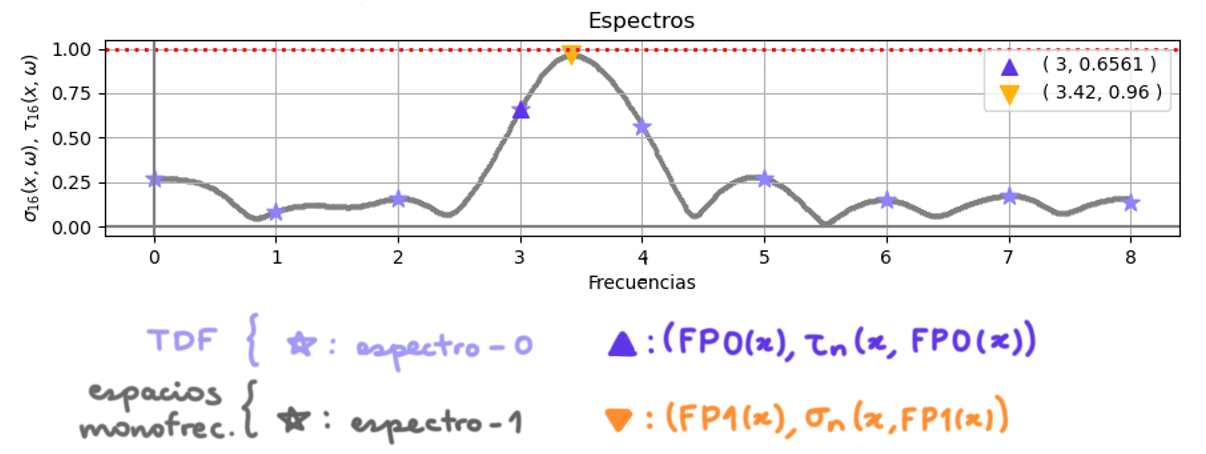
\includegraphics[scale = 1.3]{./estudios_espectrales/ejemplo_comparacion_1}
\end{figure}


Observe cómo el espectro-$1$ parece completar la información
dada por el espectro-$0$, pues, a diferencia del primero,
el espectro-$0$
da coeficientes de frecuencia $\tau_{n}(x, \omega)$ sólo
para algunas frecuencias enteras $\omega$, mientras que en el espectro-$1$
es posible considerar cualesquiera frecuencias $\omega \geq 0$; como puede observar
en la gráfica, 
\[
FP0 (x) = 3 \hspace{0.2cm} \textit{y} \hspace{0.2cm}
FP1 (x) = 3.38;
\]
esta segunda frecuencia es mucho más cercana al valor
real de la frecuencia $\omega =3.4$ del sinusoide del que
fue obtenida la señal $x$; como agregamos ruido en las mediciones, no se
obtuvo exactamente $FP1(x) = 3.4$, aunque si no
hubiésemos agregado ruido en el muestreo, sí hubiésemos obtenido
que la frecuencia principal-$1$ es $3.4$ (siempre y cuando
$3.4 \in Dom_{\omega}$). \\

A pesar de que el espectro-$0$, el obtenido a partir de la
transformada discreta de Fourier, no dio una mala estimación (del rango
de frecuencias $Dom_{TDF,n}$ considerado por esta herramienta
$\omega =3$ es el valor más cercano al valor real $\omega = 3.4$), vemos en este
ejemplo que usando el espectro-$1$ de una señal con una malla de
frecuencias $Dom_{\omega} \supseteq Dom_{TDF,n}$
suficientemente densa, es posible obtener mejores
estimaciones de frecuencias que modelen a la señal original. \\

Mostramos ahora la gráfica de $x$ junto con
\begin{itemize}
	\item la parte de la síntesis de $x$ respecto a la $TDF$
	que corresponde a la frecuencia principal
	$FP0(x)$, 
	\begin{figure}[H]
			\sidecaption{
			\label{fig: comparacion 2}
			}
			\centering
			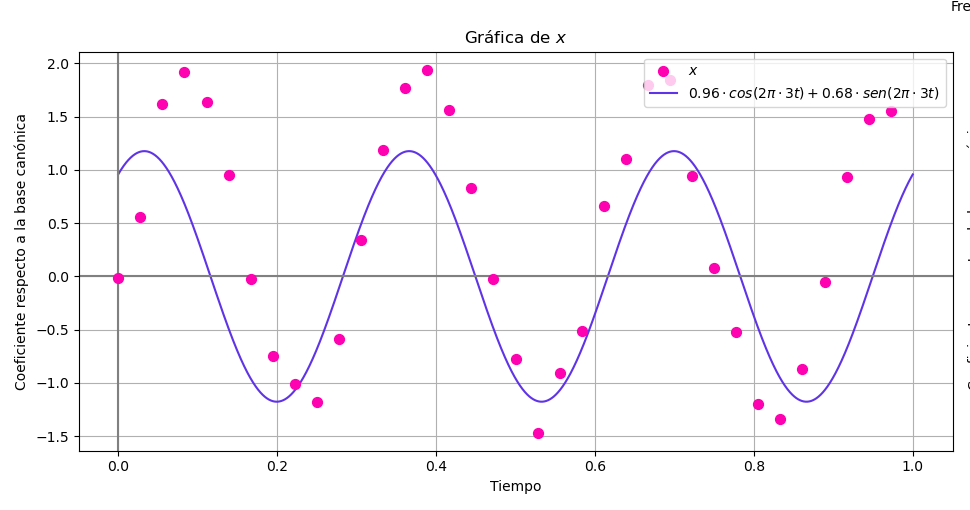
\includegraphics[scale = 0.5]{./estudios_espectrales/ejemplo_comparacion_2} 
		\end{figure}		
	
	y
	\item la señal $\Pi_{P_{16, 3.42}}(x)$, o sea, la señal de
	dimensión $16$ y frecuencia $FP0(x)$ más cercana a $x$, junto con
	el sinusoide continuo del que fue muestreado.
	\begin{figure}[H]
			\sidecaption{
			Para obtener la versión continua del sinusoide 
			discreto $\Pi_{P_{16, 3.42}}(x)$ (i.e. la gráfica naranja),
			usamos las fórmulas establecidas en los teoremas
			\ref{teo: amelie1} y \ref{teo: amelie2}.
			\label{fig: comparacion 3}
			}
			\centering
			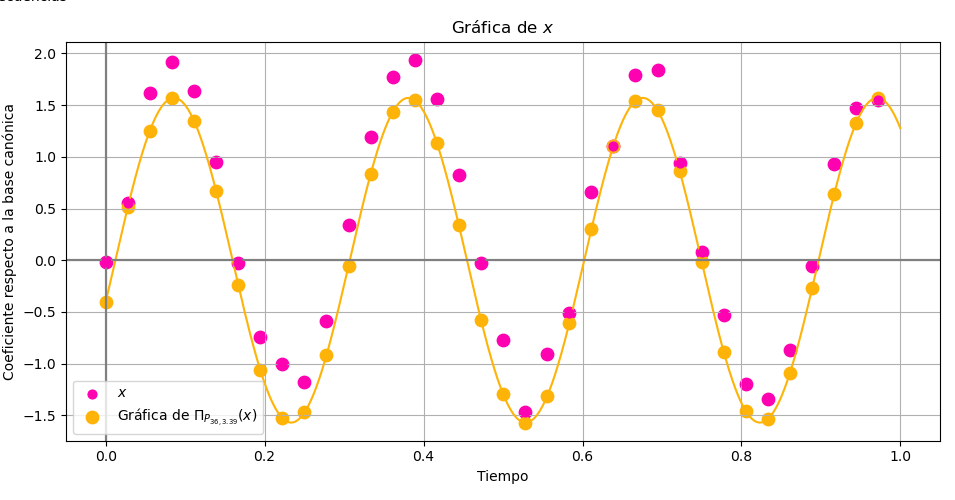
\includegraphics[scale = 0.5]{./estudios_espectrales/ejemplo_comparacion_3} 
		\end{figure}		
\end{itemize}


Note que el sinusoide naranja en 
\ref{fig: comparacion 3}
parece ajustarse mucho mejor a la gráfica de $x$
que el sinusoide morado en la figura 
\ref{fig: comparacion 2};
est era de esperarse, pues
el sinuside morado no es más que un sumando 
de la síntesis de $x$ para expresar a la
señal $x$ como una suma ponderada de sinusoides
(c.f.\TODO{nota}), por lo que faltaría considerar
a los demás sinusoides para obtener una gráfica que, de hecho, ajuste
perfectamente los puntos de la gráfica de $x$
(c.f. ejemplo \ref{ej: DFT1}), mientras que el sinusoide
naranja no sólo tiene frecuencia igual a 
$FM1(x)$, sino que es el representante de esta 
frecuencia que minimiza su distancia euclidea a $x$.

\final
\end{ejemplo}